\documentclass[12pt]{article}
\usepackage[margin=1in]{geometry}
\usepackage{amsthm,amssymb}
\usepackage{amsmath}
\usepackage{bbm}
\usepackage{amsfonts}
\usepackage{amssymb}
\usepackage{physics}
\usepackage[round]{natbib}
\bibliographystyle{plainnat}
\newcommand{\N}{\mathbb{N}}
\newcommand{\R}{\mathbb{R}}
\newcommand{\Z}{\mathbb{Z}}
\newcommand{\Q}{\mathbb{Q}}
\newcommand{\matr}[1]{\mathbf{#1}}
\newenvironment{theorem}[2][Theorem]{\begin{trivlist}
\item[\hskip \labelsep {\bfseries #1}\hskip \labelsep {\bfseries #2.}]}{\end{trivlist}}
\newenvironment{lemma}[2][Lemma]{\begin{trivlist}
\item[\hskip \labelsep {\bfseries #1}\hskip \labelsep {\bfseries #2.}]}{\end{trivlist}}
\newenvironment{exercise}[2][Exercise]{\begin{trivlist}
\item[\hskip \labelsep {\bfseries #1}\hskip \labelsep {\bfseries #2.}]}{\end{trivlist}}
\newenvironment{problem}[2][Problem]{\begin{trivlist}
\item[\hskip \labelsep {\bfseries #1}\hskip \labelsep {\bfseries #2.}]}{\end{trivlist}}
\newenvironment{question}[2][Question]{\begin{trivlist}
\item[\hskip \labelsep {\bfseries #1}\hskip \labelsep {\bfseries #2.}]}{\end{trivlist}}
\newenvironment{corollary}[2][Corollary]{\begin{trivlist}
\item[\hskip \labelsep {\bfseries #1}\hskip \labelsep {\bfseries #2.}]}{\end{trivlist}}


\usepackage{xspace}
\newcommand{\A}{\ensuremath{\mathcal{A}}\xspace}
\newcommand{\B}{\ensuremath{\mathcal{B}}\xspace}
\newcommand\pa[1]{\ensuremath{\left(#1\right)}}

%For the infografic
\usepackage{tikz,times}
%\usepackage[paperwidth=25cm,paperheight=22cm,left=1cm,top=1cm]{geometry}
\usetikzlibrary{mindmap,backgrounds}
\usepackage{xcolor}
\usepackage{color}

% Example: download a usepackage 
%\usepackage{CJK}


% For the code
\usepackage{listings}
\usepackage{pythonhighlight}


% for tables
\usepackage{adjustbox}
\usepackage[flushleft]{threeparttable}
%\usepackage[labelfont=sc]{caption}





\begin{document}

\definecolor{bitter}{rgb}{1.0, 0.46, 0.09}
\definecolor{redalt}{rgb}{0.65, 0.0, 0.0}
\definecolor{citrine}{rgb}{0.9, 0.9,0}

\title{Problem Set 5}
\author{Jonathan Tregde\\
ECON815: Topics in Microeconomics}
\date{Fall 2019}
\maketitle
\begin{question}{1} Description of Economic Question

A common debate among researchers in monetary theory and policy is discretion versus policy rules. \cite{Taylor1993} introduced the now-famous "Taylor Rule," which prescribes a simple equation for calculating what the Effective Federal Funds rate should be. The equation is as follows:

\begin{align} 
r = p + 0.5y + 0.5(p-2) +2
\end{align}
where

$r =$ the federal funds rate

$p =$ the inflation rate

$y =$ the percent deviation of real GDP from a target
\vspace{5mm}

This is, of course, an example of a policy rule. The policy-makers simply set the policy based on the data. Discretion, however, allows policy-makers to deviate from a set rule. They may perhaps use a rule to guide them, but the decision to change the rate or even by how much could differ from what the rule would dictate. Discretion allows policy-makers to make "threats" about potential future actions, but then renig later if they feel it is no longer optimal to act in that way.

For this assignment, I was interested in analyzing how closely the Federal Reserve is following the Taylor Rule.

\end{question}

\begin{question}{2} Description of Data

For this assignment, I used FRED data which included the effective Federal Funds rate, real GDP per capita, potential GDP, and the GDP deflator, which was used as a measure of inflation. All of the series except for the Federal Funds rate are measured quarterly, while the Federal Funds rate is monthly. Because of this, I took the quarterly average of the Federal Funds rate and used this so all the data was of the same frequency.

Next, I calculated the percent change in inflation and the percent deviation of GDP from the target, which in this case is potential GDP. I then used these to calculate the "Taylor Rule" interest rate, which can be used to compare to the Effective Federal Funds Rate.


\end{question}
\newpage


\begin{question}{3} Visualizations

I begin by plotting the Federal Funds Rate (FFR) against inflation, as maintaining low inflation is part of the dual mandate the Federal Reserve has been charged with, and thus should be an influence in their policy.
\begin{figure}[!h]
\centering
\caption{\textsc{Effective Federal Funds Rate vs. Inflation}}
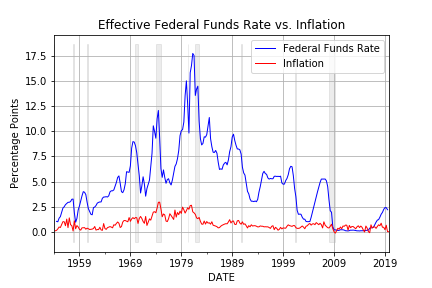
\includegraphics[scale=0.6]{inflfed_graph.png}
\end{figure}

As is evident by the graph, spikes in inflation do indeed spur movement in the FFR. A prime example is the drastic rate hikes during the early 1980s as part of an effort to squash relatively high inflation. However, it is also evident, that inflation is not the whole story behind changes in the FFR.

Next, I plot the FFR along with the "Taylor Rule" Rate. As defined above, the "Taylor Rule" Rate is not only determined by inflation, but also the output gap between GDP and the target.
\begin{figure}[!h]
\centering
\caption{\textsc{Effective Federal Funds Rate vs. Taylor Rule Rate }}
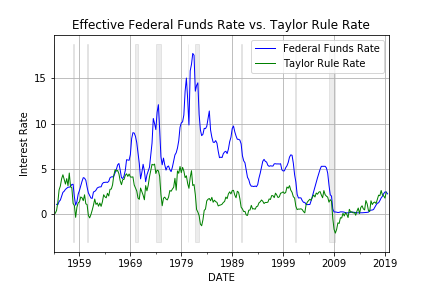
\includegraphics[scale=0.6]{fed_tr_graph.png}

\end{figure}

This plot clearly shows that the Taylor Rule is closer to determining the FFR than inflation alone. However, it is still not a one-to-one match, even after 1993 when the rule was proposed. (I would also like to note, that I believe there was an issue with my calculation of the "Taylor Rule" since the two lines should be much closer throughout the '80s and '90s based on other graphs I have seen.)

Finally, I plot the difference in the FFR and the "Taylor Rule" Rate in an effort to show periods of divergence and convergence of the two rates.

\begin{figure}[!h]
\centering
\caption{\textsc{Difference Between FFR and the "Taylor Rule" Rate}}
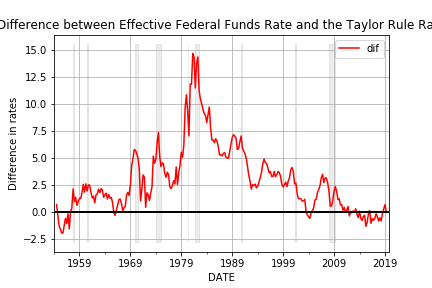
\includegraphics[scale=0.6]{difplot_graph.png}

\end{figure}

\end{question}
\newpage

\begin{question}{4} Econometric Model

Now, for the econometric model, I begin with a simple OLS model which is as follows:
\begin{align}
\nonumber
r_t = \alpha_t + {\beta}_t*y_t + {\gamma}_t*p_t
\end{align}
with $r$, $y$, and $p$ defined as above.

The results from this estimation are reported here:

% latex table generated in R 3.6.1 by xtable 1.8-4 package
\begin{table}[ht]
\centering
\begin{tabular}{rrrrr}
  \hline
 & Estimate & Std. Error & t value & Pr($>$ $|$t$|$) \\ 
  \hline
(Intercept) & 1.5501 & 0.2994 & 5.18 & 0.0000 \\ 
  y & 0.1170 & 0.0732 & 1.60 & 0.1109 \\ 
  p & 4.4011 & 0.2890 & 15.23 & 0.0000 \\ 
   \hline
\end{tabular}
\end{table}

I next use the "Taylor Rule" as a determinant of the FFR, and include an indicator for the US being in a recession, as this also affects monetary policy decisions, though is itself endogenous since recession status is defined by GDP falling for two consecutive quarters.

% latex table generated in R 3.6.1 by xtable 1.8-4 package
\begin{table}[ht]
\centering
\begin{tabular}{rrrrr}
  \hline
 & Estimate & Std. Error & t value & Pr($>$ $|$t$|$) \\ 
  \hline
(Intercept) & 2.2548 & 0.3162 & 7.13 & 0.0000 \\ 
  Taylor Rule & 1.3124 & 0.1289 & 10.18 & 0.0000 \\ 
  Recession & 2.9953 & 0.5601 & 5.35 & 0.0000 \\ 
   \hline
\end{tabular}
\end{table}

This table shows that both the Taylor Rule and the recession indicator are positive and significant. We might expect the coefficient on the Taylor Rule to be close to 1 if the FFR followed the Taylor Rule exactly. At any rate, these results show that there is a positive correlation between the Taylor Rule and the FFR. I'll use caution in taking too much away from this result, though, because the adjusted $R^2$ for this model was only 0.34, which means that only about 34\% of the variation in the FFR is accounted for by this estimation.

\end{question}
\newpage

\bibliography{PS5bib}


\end{document}
